\clearpage
\section{镜中灯条边缘的闪点}
相机正对一面光滑的镜子。沿着某个像素看过去，视线碰到镜面后只有一个反射方向。只要相机、镜子和灯牌都没动，每次沿这个方向找到的也应当是灯牌上的同一点。第一版已经能在镜子里画出相机背后的灯牌，橙色亮条旁却散着细小的亮点。为了分清它来自镜面还是相机，我们做了两组检查。

\begin{figure}[H]\centering
\begin{minipage}{.40\linewidth}\centering
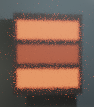
\includegraphics[height=32mm]{../../../output/profiling/scene-reflections/mirror-edge-before.png}\\
{\small 镜面也随机取方向}
\end{minipage}\hfill
\begin{minipage}{.55\linewidth}\centering

\includegraphics[height=32mm]{../../../output/profiling/scene-reflections/mirror-edge-after.png}\\
{\small 粗糙度为零时，沿几何反射方向取色}
\end{minipage}
\caption{从正式编辑器第 24 帧截取的同一区域，均已开启 TAA。两版使用同一面镜子，材质粗糙度都为零。RenderDoc 读回的颜色在计算倒影前逐字节相同。}
\end{figure}

另一组试验固定相机和像素内的取样位置，直接读取倒影着色器的结果。在 $96\times96$ 的图上连续画 16 帧，将每个像素与它在第一帧的颜色作比较。三个通道的变化合成一个数，即 $\sqrt{(\Delta R)^2+(\Delta G)^2+(\Delta B)^2}$。旧版最大差为 4.03113。这是送往显示器之前的线性颜色。亮条的 RGB 是 $(4,0.48,0.14)$，它和黑色之间的距离约为 4.03。这说明有像素前一帧取到了亮条，后一帧却取到了黑色。

在 \path{ScreenSpace/Shaders/StochasticSSR.comp} 中，旧版对每种材质都执行下面的第一行。即使粗糙度为零，用来决定反射方向分布宽度的 $a$ 仍至少是 0.002。下一帧换了随机数，射线就可能落在灯条边缘的另一侧。

\begin{Code}
// 旧版对镜面和粗糙材质都用这个宽度取样。
float a = max(.002, roughness * roughness);
\end{Code}
新版在同一文件的 \code{sampleReflection} 中先处理光滑镜面。\code{v} 从表面指向相机，\code{n} 是表面法线。其余材质继续按粗糙度取样。
\begin{Code}
if (roughness == 0.)
    direction = reflect(-v, n); // 相机的视线碰到镜面后沿这个方向继续。
\end{Code}
重复 16 帧的检查，粗糙度为零时最大颜色差降到 0。另把粗糙度设为 0.55，条纹仍然会散开。\href{run:../profiling/scene-reflections/test-stability.csv}{连续帧读数}\quad
\href{run:../profiling/scene-reflections/test-method.md}{试验与截帧方法}
